\chapter{Study and analysis method}\label{chap:4}

\section{Participants and study scope}\label{sec:4-1}

The study involved six dyads, identified as G01--G06, with twelve participants identified consistently as P01--P12. All pairs were already friends and had worked together; most were also members of a current course group, according to the researcher's final background clarification. Relationship duration and cooperation frequency were not measured. The study therefore describes collaboration between familiar partners. [\hyperlink{src:D18}{D18}]

Eight participants had previously used VR and four had not, according to the completed background record. One G05 participant had taken part in a Tangram club more than a decade earlier; the others were reported to have no Tangram experience. These reports describe prior exposure rather than current expertise. Participant numbers are retained across physical and VR conditions; viewing position is not used as a participant identity. [\hyperlink{src:D18}{D18}]

The study used an exploratory comparison with one designated process per pair and condition. All six pairs are included. Practice, restarts and additional experiences are recorded in the session history. G02's VR videos were recorded in a later session using previously unattempted target patterns, so the recorded tasks did not repeat a known solution. Their questionnaires describe the original session and are analysed as condition-level responses rather than ratings of individual recorded episodes. [\hyperlink{src:D17}{D17}, \hyperlink{src:D74}{D74}]


\section{Task and actual procedure}\label{sec:4-2}

Tangram provided a common task in which partners could refer to the same pieces, inspect a changing arrangement and decide together how to proceed. Retaining this task across the physical and VR arrangements kept the comparison focused on viewing and interaction within a common problem. Free manipulation allowed the pair to organise work at the level of a piece or local part, including changes between separate attempts and joint adjustment. This follows the interest in shared problem states and changing divisions of work described in collaborative learning and workspace-awareness research \cite{roschelle1995,dillenbourg1999,gutwin2002}. [\hyperlink{src:D72}{D72}, \hyperlink{src:D33}{D33}, \hyperlink{src:D36}{D36}, \hyperlink{src:D69}{D69}, \hyperlink{src:D38}{D38}]

Participants used seven Tangram pieces to construct target silhouettes. Both could manipulate the pieces, communicate naturally and decide how to divide work. The procedure did not assign a director or operator and did not require continuous think-aloud speech. Individual questionnaires followed the research rounds, and a recorded dyadic interview provided retrospective accounts. [\hyperlink{src:D38}{D38}]

All dyads experienced the conditions in the same order: R01, physical direct viewing; R02, physical overhead video; R03, first-person VR; and R04, shared overhead VR. Target patterns differed across rounds and were not balanced for difficulty. In G05, the chair was selected as a harder task after the pair performed well earlier. Comparisons therefore concern the task and viewing arrangements as implemented, including order, practice and pattern differences. [\hyperlink{src:D17}{D17}, \hyperlink{src:D44}{D44}]

The apparatus and viewing-to-action mapping are shown in Figure~\ref{fig:3-2}. R02 used three smartphones connected through Discord and barriers that blocked direct sight of the pieces. R03 and R04 used two networked Quest 3 headsets. In R04 the head-following display showed the world-fixed overhead image, while tracked controllers continued to operate in the shared virtual workspace. Section~\ref{sec:3-2} gives the full arrangement. [\hyperlink{src:D24}{D24}, \hyperlink{src:D47}{D47}, \hyperlink{src:D41}{D41}]

Familiarisation followed different entry criteria. Participants with VR experience could proceed when they felt ready. Novices were asked to complete a pattern and switch viewpoints during practice. Practice duration and control proficiency were therefore not standardised across participants. G04's two woman attempts preceded the formal overhead swimmer task as adaptation. G06's same-side positioning began during familiarisation before the formal first-person round. [\hyperlink{src:D18}{D18}, \hyperlink{src:D45}{D45}, \hyperlink{src:D14}{D14}]

The researcher reports that changes of participant position were self-initiated. Researcher intervention is recorded separately where it occurred. G04's physical direct round included structural feedback, encouragement to communicate and later confirmation of an earlier approach before the pair abandoned the task. G03's overhead chair included two structural hints before completion. Elsewhere, no-hint status follows the researcher's declaration; the absence of a hint in a log is not an independent audio verification of its absence. [\hyperlink{src:D46}{D46}, \hyperlink{src:D07}{D07}, \hyperlink{src:D59}{D59}]

Participants were instructed to use all seven pieces and match the target silhouette. After they announced completion, the researcher checked the configuration on site. A solution could be accepted with an internal partition different from the reference image. The analysis records this on-site judgment separately from subsequent geometric checking. Selected configurations were reconstructed during analysis to examine their outlines; the researcher identified a mismatch in the accepted G06 first-person candle while reviewing it as a focal observation, and reconstruction was used to check that observation. [\hyperlink{src:D18}{D18}, \hyperlink{src:D16}{D16}]


\section{Evidence corpus and provenance}\label{sec:4-3}

Data collection combined process records with participants' accounts because the study concerned both how collaboration developed and how it was experienced. Recordings and available system traces retained placements, responses and changes in control. Post-round ratings described particular aspects of the experience, and the final interview allowed participants to explain difficulties and decisions in their own terms. This combination followed the planning emphasis on behavioural activity, with completion measures used as context for understanding the task process. [\hyperlink{src:D36}{D36}, \hyperlink{src:D70}{D70}, \hyperlink{src:D73}{D73}]

The corpus is organised as six dyads across four research conditions, giving 24 group--condition cells. The completed source queue contains 26 researcher process reports, including multiple recordings or endpoints for some processes. This is a count of source reports, not independent trials. The reports cover all 24 cells, including the later G02 recordings on new target patterns. [\hyperlink{src:D17}{D17}]

The analysis combines researcher-prepared video observations and corrections, recordings of the task, six group interview texts, 48 confirmed post-round questionnaire responses and available Unity records. Video observations describe visible placements, body positions and how participants continued one another's work. VR event and pose records support the timing, piece identity and sequence of recorded manipulations. Interview text provides participants' retrospective accounts, while questionnaires describe their experience of each round. Selected frames and log sequences were checked against the source files; these targeted checks supplement the researcher's process reports. [\hyperlink{src:D17}{D17}, \hyperlink{src:D44}{D44}, \hyperlink{src:D20}{D20}]

All six physical overhead recordings (R02) have no usable audio, so these recordings support visible-action descriptions. VR recordings generally captured only the recording participant's own voice, and the other endpoint was used where available. A missing partner voice is treated as missing audio coverage. G04's formal overhead swimmer round is covered by \href{https://github.com/YiyangQin-UQ/REIT7841/blob/main/thesis/v1.1/materials/README.md\#d67}{V23} but not by the surviving \href{https://github.com/YiyangQin-UQ/REIT7841/blob/main/thesis/v1.1/materials/README.md\#d66}{V17} segment, and G06 has no recording from the other endpoint. Spoken content from researcher reports is presented as attributed paraphrase unless its wording and speaker have been checked. [\hyperlink{src:D19}{D19}]

The six interview texts combine speakers and contain transcription errors. The analysis uses group-level paraphrases where individual attribution cannot be established. Answers to questions about imagined viewing conditions are treated as participants' reflections on those scenarios. Supervisor correspondence and meeting transcripts inform the design history and rationale rather than the behavioural findings. [\hyperlink{src:D19}{D19}, \hyperlink{src:D44}{D44}]

\par\addvspace{8pt}
\noindent\begin{minipage}{\linewidth}
\begingroup
\centering
\setstretch{1}
\fontsize{10}{12.3}\selectfont
\setlength{\tabcolsep}{2.2pt}
\renewcommand{\arraystretch}{1.18}
\captionof{table}[Coverage of process reports and confirmed questionnaires.]{Coverage of process reports and confirmed questionnaires.}\label{tab:4-1}
\begin{tabular}{@{}>{\raggedright\arraybackslash}p{13.459mm}>{\raggedright\arraybackslash}p{45.183mm}>{\raggedright\arraybackslash}p{31.724mm}>{\raggedright\arraybackslash}p{34.608mm}>{\raggedright\arraybackslash}p{28.840mm}@{}}
\toprule
\textbf{Round} & \textbf{Condition} & \textbf{Dyads with process reports} & \textbf{Confirmed questionnaires} & \textbf{NA item entries} \\
\midrule
R01 & Physical direct & 6 & 12 & 1 \\
\addlinespace[3pt]
R02 & Physical overhead video & 6 & 12 & 1 \\
\addlinespace[3pt]
R03 & First-person VR & 6 & 12 & 0 \\
\addlinespace[3pt]
R04 & Shared overhead VR & 6 & 12 & 0 \\
\bottomrule
\end{tabular}
\par\endgroup
\end{minipage}\par\addvspace{8pt}

The 26 source reports cover 24 pair--condition cells. The two NA item values are Q01 for P08 in R01 and R02.


\section{Questionnaire and system records}\label{sec:4-4}

The questionnaire contains twelve study-specific items rated from 1 to 5, with an unable-to-judge or not-applicable option. The items cover identifying referred pieces, understanding intended locations, judging a partner's understanding, explaining locations, following partner activity, task progress, action timing, avoiding interference, movement, rotation, responsibility and solving together. They are interpreted separately. They are not a validated composite collaboration scale. Appendix B gives the full item wording and the item-level data. [\hyperlink{src:D20}{D20}]

The questionnaire dataset contains 48 confirmed responses: twelve participants each contributed answers for all four rounds. Forty-five responses came from the original export. For the remaining three, the researcher reported that the participants had confirmed their answers for the corresponding round were identical to the referenced response, and entered those confirmed values. The confirmation record preserves which response was used and when the clarification was recorded; the historical submission timestamps were retained. The two original not-applicable entries remain non-numeric. All 48 confirmed responses are included in the descriptive tables and figures. [\hyperlink{src:D20}{D20}]

Questionnaire comparisons were made item by item, first within each participant across rounds and then between partners. The twelve study-specific items were kept separate, with no composite collaboration score or significance testing. Ratings are used alongside the process records to describe the experience of a round; a round-level response is not assigned to a single episode within it. Appendix B provides the full item wording and confirmed values. [\hyperlink{src:D44}{D44}, \hyperlink{src:D20}{D20}]

The VR records were first segmented into software attempts using start, reset, pause, resume and end events. Each selected attempt was then linked to a research condition through its task, viewing condition and video--log anchors. Software round numbers were kept separate from R01--R04. For example, G06's retained overhead process is software R03 after an interrupted software R02, but remains research condition R04. Filenames containing TECHNICAL\_TEST were retained as recorded; the filename alone was not used to identify the dyad or decide whether a process was formal. [\hyperlink{src:D17}{D17}, \hyperlink{src:D15}{D15}, \hyperlink{src:D25}{D25}]

The collection-period V3 logging guide describes accepted grabs, movement onset, piece poses, release and post-release settling. Round-start metadata in the available revised-version logs specify approximately 10 Hz piece-pose sampling and 2 Hz participant-pose sampling, with a movement-onset threshold of 2 mm or 2 degrees. These are nominal logging settings; actual samples follow the recorded timestamps. Participant poses describe head and controller positions and orientations, rather than eye gaze. After release, the stream includes settling poses and a terminal event labelled stable\_0.3s or settle\_timeout\_2s. The timeout marks the end of the observation window and does not establish that the piece had become stationary. [\hyperlink{src:D25}{D25}]

For action timelines, each grab\_accepted event was paired with its piece\_release using the software round, piece ID and manipulation ID, and the endpoint identity and temporal order were checked. Requests, denied grabs and repeated selections were not counted as new successful holds. Forced release and interruption records were kept distinct from an ordinary release. The selected intervals were checked against the corresponding original CSV rows. They show when an endpoint held a piece; their duration and count do not measure understanding, effort or the value of a contribution. [\hyperlink{src:D25}{D25}, \hyperlink{src:D21}{D21}]

A configuration at an analysis time was reconstructed from the latest recorded pose for each piece at or before that time within the selected attempt. Eligible states came from initial placement, held-pose, release, settling-pose and settled records. This last-known-state rule retains post-release changes and avoids interpolating an unrecorded placement. The source event, row and age of each pose were kept with the reconstruction, and later events were checked before treating a selected state as persistent. A missing later update means no later change was recorded for that piece in the selected trace. [\hyperlink{src:D26}{D26}]

Video position, active task seconds and UTC or wall-clock time were retained as separate clocks. Pauses, resets and delayed manual ending were read from the software record. Distinctive visible manipulations and task boundaries provided local alignment anchors, with mappings stated for the selected case. For G06 and G03, repeated visible grabs were matched to the event records to establish the participant mapping. G03's P05 event reported at video 03:06 and the selected active-time log sequence retain their separate timestamps. This preserves the distinction between identifying the person and aligning a particular event. [\hyperlink{src:D21}{D21}, \hyperlink{src:D26}{D26}, \hyperlink{src:D06}{D06}]


\section{Analytic procedure and interpretation}\label{sec:4-5}

\begin{figureunit}{4-1}
Analysis began within each dyad and condition and followed connected episodes rather than isolated grabs. An episode began with a proposal, placement or problem relevant to the current arrangement, and followed the partner's response, subsequent manipulation and resulting configuration until the local issue changed, was resolved or was abandoned. The record separated the accessible view and target, who proposed and built a part, who later changed it, the before-and-after arrangement and the source of any correctness judgment. This attention to unfolding talk, action and artefacts was informed by interaction analysis \cite{jordan1995}. Figure~\ref{fig:4-1} summarises the analysis workflow. [\hyperlink{src:D44}{D44}, \hyperlink{src:D21}{D21}]

\par\begingroup
\centering
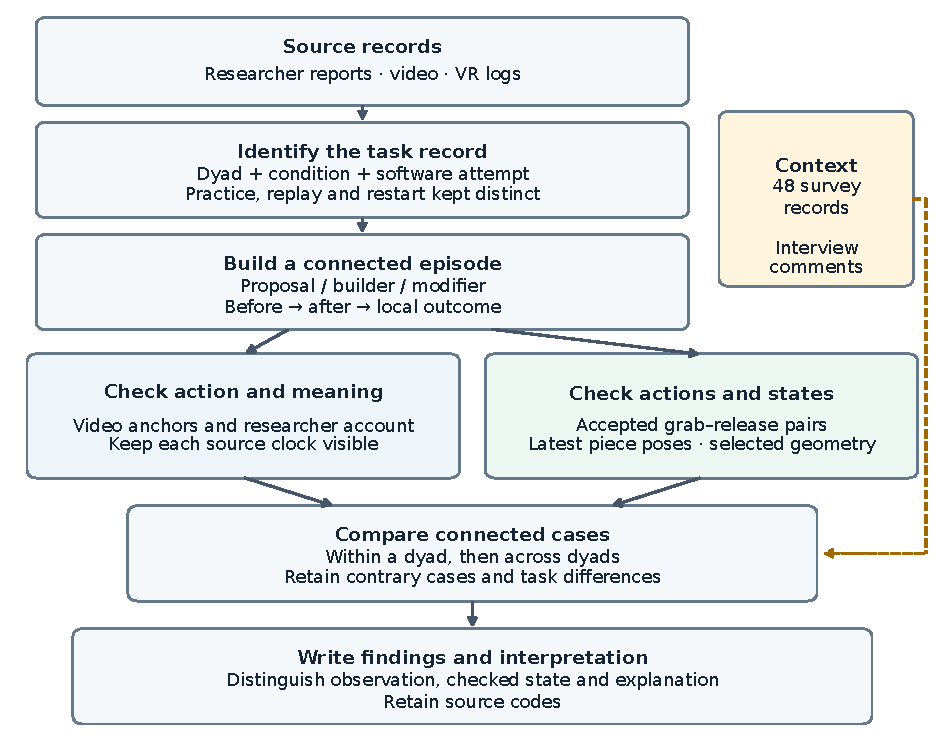
\includegraphics[width=\linewidth,height=125mm,keepaspectratio]{assets/figures/Figure4_1_analysis_flow.pdf}
\captionof{figure}[Analysis workflow.]{Analysis workflow. Source identification precedes episode construction so that software attempts, research conditions and recording sessions are identified consistently. Video and researcher accounts describe the meaning and order of local actions; accepted event pairs and reconstructed states check selected movements and configurations. Questionnaire responses and interview comments provide context for the case comparison. The separation between source-specific clocks, on-site acceptance and later geometric verification is retained in the findings.}\label{fig:4-1}
\par\endgroup
\end{figureunit}

Researcher observations and subsequent corrections provided the initial event accounts. Selected video frames and log intervals were then checked to examine the reported order of actions, the pieces involved and the resulting arrangement. Grounding and workspace awareness served as sensitising concepts when interpreting reference, response, coordination and assistance \cite{clark1991,gutwin2002}. The operational distinctions in Appendix C describe local uptake, parallel and complementary work, preservation, self-revision, partner revision and manipulation difficulty. Table~\ref{tab:C-2} shows three worked applications with their original time bases. [\hyperlink{src:D44}{D44}, \hyperlink{src:D21}{D21}]

Processes were compared first across conditions within a dyad and then across dyads. Cases were selected for detailed presentation when the relevant sequence could be traced and when they clarified a question raised by the other records. These included configurations that looked plausible during the task, shifts in who developed a part, preservation of a partner's arrangement, self-revision and active partner intervention. G06's candle connects configuration change with shared rebuilding; G01 and G03 provide distinct self-revision sequences. Action and response support an interpretation of a local step, while an intention or reason for preserving it requires the surrounding account. [\hyperlink{src:D17}{D17}, \hyperlink{src:D21}{D21}]

The comparison across pairs used a process criterion: participants formed an arrangement that resembled the target as a whole while a piece remained unused, or while the contour or proportions still differed from the target after all seven pieces had been used. Ordinary unfinished search and difficulty placing an individual piece were recorded separately. Each pair contributed one presence judgment per condition. The researcher identified this pattern in three of six first-person VR records and in none of the six shared-overhead VR records. Table~\ref{tab:A-3} links each pair to the relevant records. [\hyperlink{src:D27}{D27}, \hyperlink{src:D74}{D74}]

The geometric checks were conducted after data collection. For selected VR states, the saved Unity piece meshes and scale were combined with the logged world positions and quaternion rotations. Vertices were projected onto the tabletop x--z plane and reduced to a convex hull for each piece, preserving the recorded arrangement and the mesh's rounded geometry. The saved scene supplied the mesh geometry, while the CSV supplied the pose at each time. Comparison panels retained a common world scale and used rigid alignment of whole arrangements. They were checked alongside the target image, video frames and process reports. [\hyperlink{src:D26}{D26}, \hyperlink{src:D16}{D16}]

For the candle comparison, the researcher first noticed that the accepted construction's outline differed from the target. Reconstructed top views placed the target and recorded configurations in a common orientation so that this difference could be inspected. A simple comparison of corresponding upper and lower spans was used as a supporting check: they are equal in the target and in the two-large-triangle layouts, whereas G06's lower span is wider. The reconstruction preserves each piece's recorded position and rotation. Numerical measurements and processing details are retained with the figure sources. [\hyperlink{src:D26}{D26}, \hyperlink{src:D16}{D16}, \hyperlink{src:D74}{D74}]

The researcher identified the focal observations, selected the cases and developed the interpretations from the study records. AI-assisted processing helped check selected sequences and geometric relations, organise the source material and prepare figures and prose. The G06 outline mismatch was an observation made by the researcher and subsequently checked through reconstruction. [\hyperlink{src:D44}{D44}, \hyperlink{src:D21}{D21}, \hyperlink{src:D74}{D74}]




\section{Consent and research assistance}\label{sec:4-6}

The study was undertaken as an educational activity for the thesis course. Twelve completed participant consent forms are retained in the local archive. In correspondence dated 6 October 2026, the supervisor confirmed that the previous testing could be used because the study had been reviewed for an educational activity rather than a research publication output. Participant codes are used in this report, and the task-image excerpts focus on the workspace and hands. [\hyperlink{src:D22}{D22}]

ChatGPT and Codex supported source organisation, English drafting and revision, log and geometric checks, programmatic figures and typesetting. The researcher conducted the study, identified the findings and judged the interpretations. The AI-use statement records this assistance by project stage. [\hyperlink{src:D23}{D23}, \hyperlink{src:D74}{D74}]


